\documentclass[12pt,a4paper]{article}

\usepackage[english]{babel}
\selectlanguage{english}
\usepackage[applemac]{inputenc}
\usepackage{graphicx}
\usepackage{xcolor}
\usepackage{fancyhdr}
\usepackage{latexsym}
\usepackage{amsfonts}
\usepackage{amssymb}
\usepackage{amsmath}
\usepackage{cite}
\usepackage{verbatim}
\usepackage{url}
\usepackage[pdftex]{hyperref}
\hypersetup{
pdfauthor={Alessandra Bonetto, Filippo Sironi, Matteo Villa},
pdfsubject={Formal Methods for Concurrent and Real-Time Systems},
pdftitle={Computer Controller Automatic Transmission},
pdfborder={0 0 0},
colorlinks,
citecolor=black,
filecolor=black,
linkcolor=black,
urlcolor=black
}
\usepackage{sans}
\usepackage{indent�rst}
\usepackage{listings}
%%
%% TRIO definition
%%
\lstdefinelanguage{TRIO}{
morekeywords=[0]{class,signature,visible,temporal,domain,domains,items,axioms,vars,formulae,end,import,modules,connections,variables,constants},
keywordstyle=[0]\color{violet}\bfseries,
morekeywords=[1]{state,event,const,TD,total,TI,direct},
keywordstyle=[1]\color{violet},
morekeywords=[2]{Dist,Past,Futr,Lasted,Lasts,Lasts_ii,Lasts_ei,WithinP,WithinF,Som,SomP,SomF,Alw,AlwP,AlwF,UpToNow,NowOn,Until,Since},
keywordstyle=[2]\color{blue},
morekeywords=[3]{integer,real},
keywordstyle=[3]\color{green},
morekeywords=[4]{all,ex,and,or,not,implies,iff},
keywordstyle=[4]\color{blue}\bfseries,
morecomment=[s][\color{green}]{/*}{*/},
morecomment=[l][\color{green}]//,
sensitive
}

\begin{document}

\thispagestyle{empty}
\begin{center}
{\huge Politecnico di Milano}
\end{center}
\begin{center}
{\huge Formal Methods for Concurrent and Real-Time Systems}
\end{center}
\vskip 9cm
\begin{center}
{\Large Computer Controller Automatic Transmission\\(Mandatory Part and Optional Part not complete yet)}
\end{center}
\vskip 2cm
\begin{center}
{\large Alessandra Bonetto\\Filippo Sironi\\Matteo Villa}
\end{center}
\vskip 2cm
\begin{center}
{\large 2009}
\end{center}

\newpage
\pagestyle{fancy}
\fancyhf{}
\fancyhead[R]{\bfseries\thepage}
\fancyhead[L]{\bfseries\rightmark}
\fancyhead[L]{\bfseries\leftmark}

\newpage
\tableofcontents

\newpage
\listoffigures

\newpage
\lstlistoflistings

\newpage\section{CCAT Class}
\label{Section:ComputerControlledAutomaticTransmission}
The \emph{ComputerControlledAutomaticTransmission} class is formalized thanks to the code reported in Listing~\ref{Code:ComputerControlledAutomaticTransmission} while Figure~\ref{Figure:CCAT} shows the \emph{big picture} of our complete designed.

\lstinputlisting[language=TRIO,tabsize=4,numbers=left,numberstyle=\small,basicstyle=\small,breaklines,breakatwhitespace,frame=single,caption=ComputerControlledAutomaticTransmission.trio,label=Code:ComputerControlledAutomaticTransmission]{../trio/ComputerControlledAutomaticTransmission.trio}

\thispagestyle{empty}
\begin{figure}[!p]
\vspace{-3 cm}
\centerline{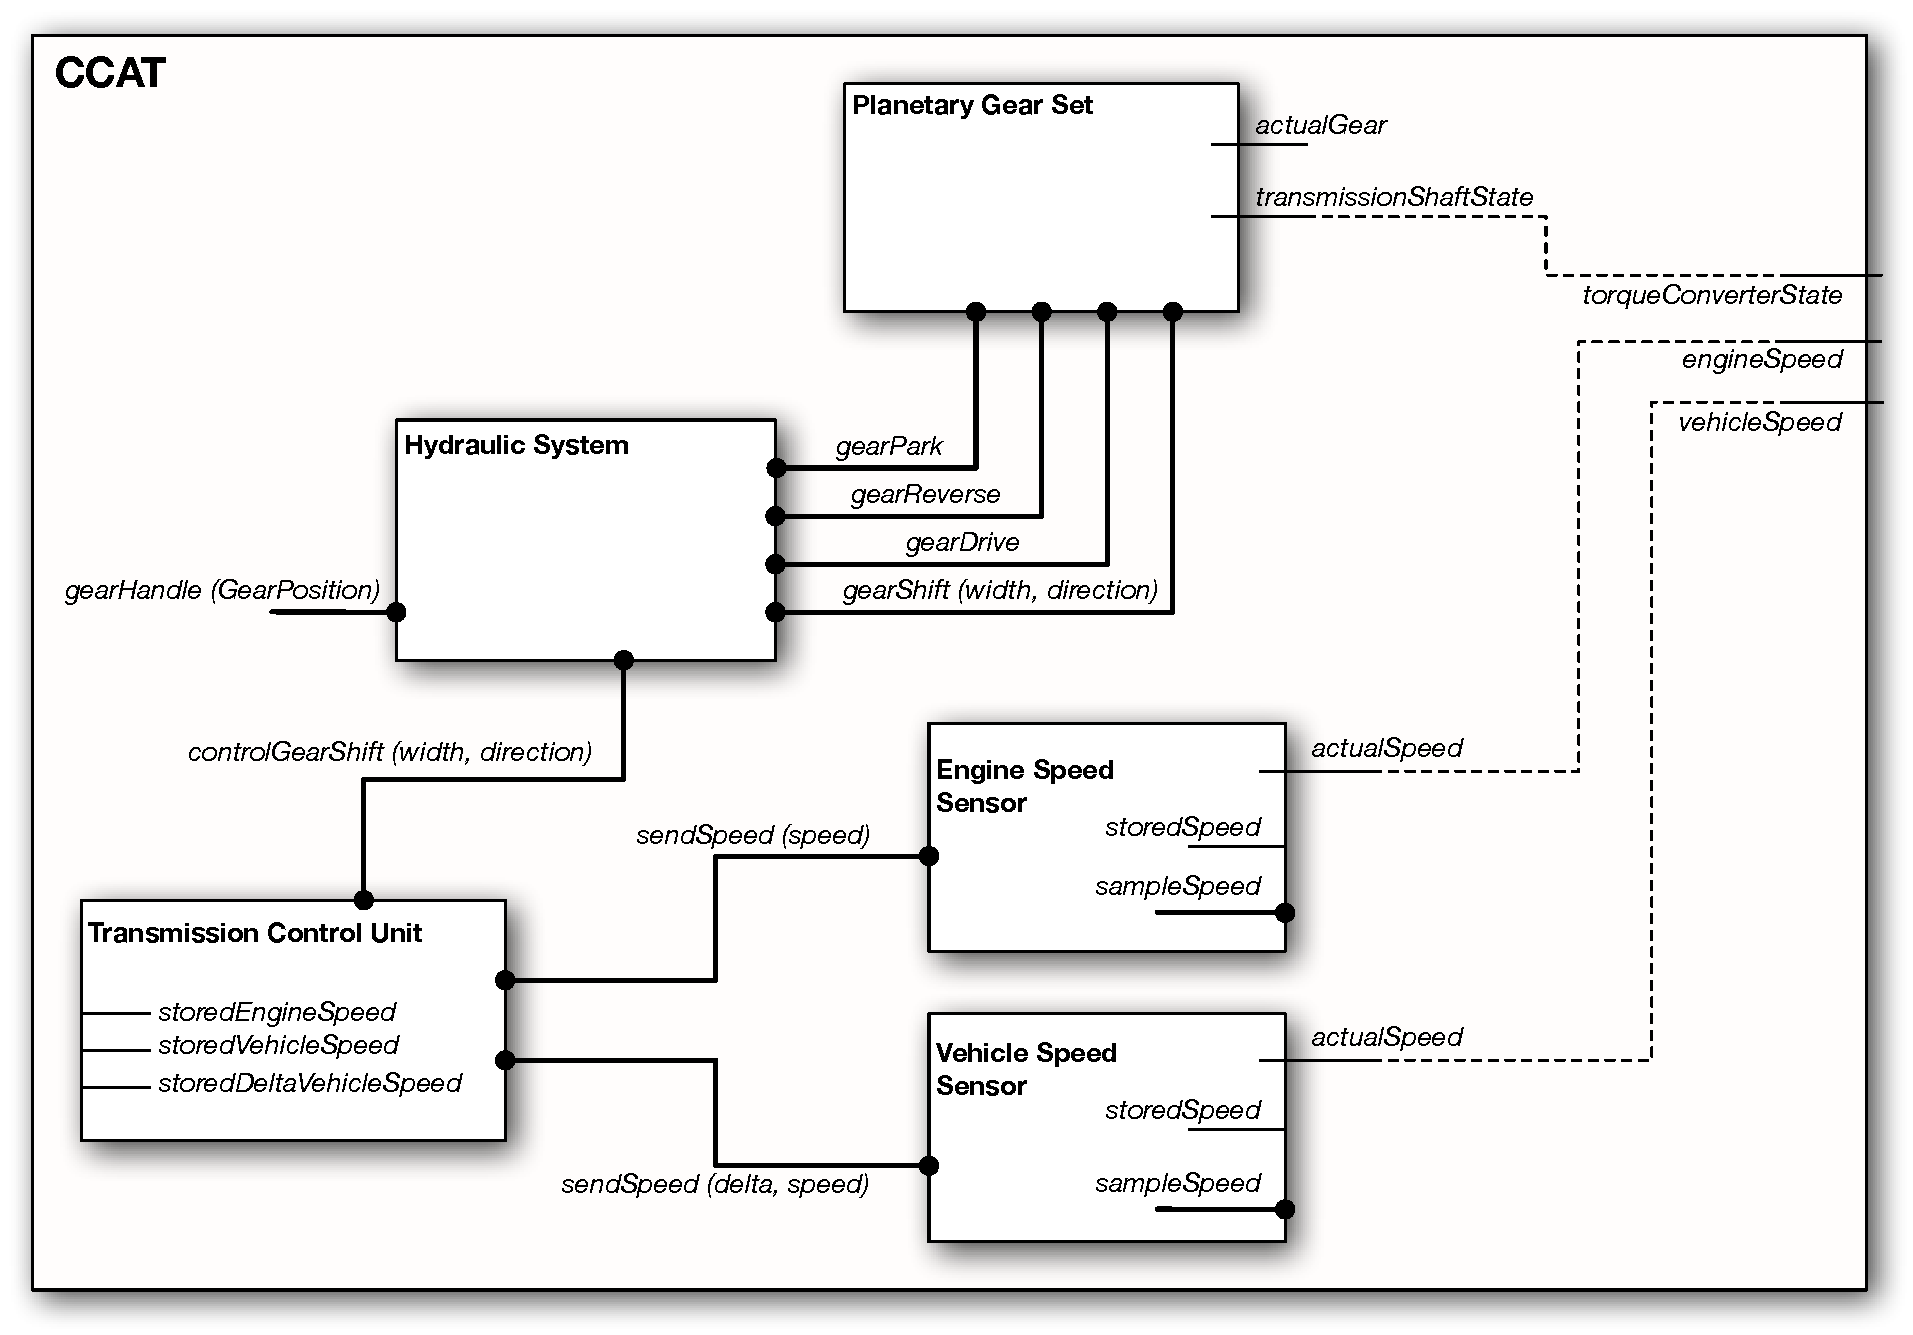
\includegraphics[scale=0.8,angle=-90]{images/CCAT.pdf}}
\caption{Computer Controller Automatic Transmission}
\label{Figure:CCAT}
\end{figure}

\newpage
Due to limitations in the verification tools we have decided to focus our verification process only on the Hydraulic System, described in Section~\ref{Section:HydraulicSystem}, and on the Planetary Gear Set, described in Section~\ref{Section:PlanetaryGearSet}.

The specification is reported in Listing~\ref{Code:ComputerControlledAutomaticTransmission2}.

\lstinputlisting[language=TRIO,tabsize=4,numbers=left,numberstyle=\small,basicstyle=\small,breaklines,breakatwhitespace,frame=single,caption=ComputerControlledAutomaticTransmission.t2p,label=Code:ComputerControlledAutomaticTransmission2]{../t2p/ComputerControlledAutomaticTransmission.t2p}

\newpage\section{Vehicle/EngineSpeedSensor Classes}
\label{Section:SpeedSensors}
The \emph{VehicleSpeedSensor} is formalized thanks to the code reported in Listing~\ref{Code:VehicleSpeedSensor} while the \emph{EngineSpeedSensor} is formalized thanks to the code reported in Listing~\ref{Code:EngineSpeedSensor}.

During the formalization of sensors we decided to simplify the design assuming that every time a \texttt{sampleSpeed} event occurs the state variable \texttt{actualSpeed} - which is \texttt{time dependent} and \texttt{total} - is automatically updated with the actual measured speed. This means we don't provide any axioms formalizing this behavior.

Moreover, we specified the starting point of the constant frequency sample chain saying that sometimes in the past there was a \texttt{sampleSpeed} occurrence. Further more, we guarantee that \texttt{sampleSpeed} events will occur at constant frequency. In addition, if the sensor has memory we imposed that the \texttt{storedValue} is equal to 0. These can be consider just like the ``initial conditions'' of the system.

At the end, we guaranteed a sensor performs the needed action if and only if a sample event occur.

We didn't write any axioms specifying the fact that a \texttt{sendSpeed} event is mutually exclusive with itself due to the \texttt{total time dependent} parameter it accepts.

\lstinputlisting[language=TRIO,tabsize=4,numbers=left,numberstyle=\small,basicstyle=\small,breaklines,breakatwhitespace,frame=single,caption=VehicleSpeedSensor.trio,label=Code:VehicleSpeedSensor]{../trio/VehicleSpeedSensor.trio}

\lstinputlisting[language=TRIO,tabsize=4,numbers=left,numberstyle=\small,basicstyle=\small,breaklines,breakatwhitespace,frame=single,caption=EngineSpeedSensor.trio,label=Code:EngineSpeedSensor]{../trio/EngineSpeedSensor.trio}

\newpage\section{PlanetaryGearSet Class}
\label{Section:PlanetaryGearSet}
The \emph{PlanetaryGearSet} class is formalized thanks to the code reported in Listing~\ref{Code:PlanetaryGearSet}.

The Planetary Gear Set guarantees that every time a gear shift event occurs the \texttt{actualGear} will be maintained until the shift is finished.

Inside this component are defined all axioms limiting gear shifts to effective ones only (e.g. it is impossibile to shift down a gear if \texttt{actualGear} is \texttt{First}.

Moreover, through the formalization of the Planetary Gear Set we impose that we can't receive a gear shift event if we are in the middle of a gear shift. Different gear shifting times are defined for different gears and different steps.

The gears \texttt{Drive}, \texttt{Park}, and \texttt{Reverse} can be selected if and only if the transmission shaft is decoupled from the engine.

The state of the Planetary Gear Set changes if and only if an event occurs.

\lstinputlisting[language=TRIO,tabsize=4,numbers=left,numberstyle=\small,basicstyle=\small,breaklines,breakatwhitespace,frame=single,caption=PlanetaryGearSet.trio,label=Code:PlanetaryGearSet]{../src/PlanetaryGearSet.trio}

\newpage\section{HydraulicSystem Class}
\label{Section:HydraulicSystem}
The \emph{HydraulicSystem} class is formalized thanks to the code reported in Listing~\ref{Code:HydraulicSystem}.

The first assumption we made before modelling the Hydraulic System was that every valve and electrovalve configuration imposes the same fluid propagation delay; this means that for every command that the Hydraulic System propagates the delay will always be the same. This behavior is formalized with the \texttt{time independent constant fluidPropagationDelay}.

The \emph{manual valve}, which permit the driver to manually select the gear mode, is modelled thanks to the \texttt{gearHandle} event and the \texttt{GearHandle} axiom. During the time in which the Hydraulic System propagate a command there can be no \texttt{gearHandle} event which somehow means the fluid propagation is faster then the driver reaction time (which is a realistic assumption).

Moreover, thanks to the \texttt{MutualExclusion} axiom, it's impossibile to generate two \texttt{gearHandle} event at the same time which means that the gear handle can't be for example in Park and Drive mode at the same instant.

\lstinputlisting[language=TRIO,tabsize=4,numbers=left,numberstyle=\small,basicstyle=\small,breaklines,breakatwhitespace,frame=single,caption=HydraulicSystem.trio,label=Code:HydraulicSystem]{../trio/HydraulicSystem.trio}

\newpage\section{TransmissionControlUnit Class}
\label{Section:TransmissionControlUnit}
The \emph{TransmissionControlUnit} class is formalized thanks to the code reported in Listing~\ref{Code:TransmissionControlUnit}.

Our first formalization of the Transmission Control Unit didn't take in account the possibility to have asynchronous sensors; the latest version of the Transmission Control Unit permits to manage asynchronous sensors thanks to internal memory modelled with three \texttt{time dependent total} values.

When handle the necessity to scale gears till the \texttt{First} with the assumption that the human reaction is way slower than sampling frequency and mechanical reactions, so, when the vehicle stops, the axiom which handle the gear scale manage to be ``active'' the necessary amount of times to scale all the gears.

The Transmission Control Unit guarantees that it doesn't raise more than one gear shift event per instant and it receives at most one event per instant from each sensor (this is described also in Section~\ref{Section:SpeedSensors} and so guaranteed in VehicleSpeedSensor and EngineSpeedSensor class).

\lstinputlisting[language=TRIO,tabsize=4,numbers=left,numberstyle=\small,basicstyle=\small,breaklines,breakatwhitespace,frame=single,caption=TransmissionControlUnit.trio,label=Code:TransmissionControlUnit]{../src/TransmissionControlUnit.trio}

\newpage\section{Annotations}
\label{Section:Annotations}
During the last phase of our modelling we decided not to formalize the \emph{Torque Converter} and this decision depends on the way the Torque Converter works.

The Torque Converter is a mechanical component that works coupling and decoupling the \emph{Transmission Shaft} and the \emph{Engine Shaft}. It solves is duty without the necessity to receive commands from any component of the system and this is the cause we have decided to remove it from our model.

Anyway, the state of the Torque Converter is really important for the system since it gives information that permits to insert or not to insert some gears and other details that aren't taken into account in this project.
\newpage\section{Properties}
\label{Section:Properties}

\begin{lstlisting}[language=TRIO,basicstyle=\small,breaklines,breakatwhitespace,frame=single,caption=Property 1,label=Code:Property1]
actualGear = First and controlGearShift (1, Up) implies Futr (actualGear = Second, fluidPropagationDelay + singleGearShiftDelay)
\end{lstlisting}

\begin{lstlisting}[language=TRIO,basicstyle=\small,breaklines,breakatwhitespace,frame=single,caption=Property 2,label=Code:Property2]
gear = Park and gearHandle (gear) and Futr (actualGear = Park, fluidPropagationDelay + parkGearShiftDelay) implies NowOn (transmissionShaftState = Detached)
\end{lstlisting}


\end{document}
